\documentclass[10pt,letterpaper]{article}
\usepackage[top=0.85in,left=2.75in,footskip=0.75in]{geometry}

% Use adjustwidth environment to exceed column width (see example table in text)
\usepackage{changepage}

% Use Unicode characters when possible
\usepackage[utf8x]{inputenc}

% textcomp package and marvosym package for additional characters
\usepackage{textcomp,marvosym}

% fixltx2e package for \textsubscript w
\usepackage{fixltx2e}

% amsmath and amssymb packages, useful for mathematical formulas and symbols
\usepackage{amsmath,amssymb}

% cite package, to clean up citations in the main text. Do not remove.
\usepackage{cite}
\usepackage{booktabs}

% Use nameref to cite supporting information files (see Supporting Information section for more info)
\usepackage{nameref,hyperref}

% line numbers
\usepackage[right]{lineno}

% ligatures disabled
\usepackage{microtype}
\DisableLigatures[f]{encoding = *, family = * }

% Text layout
\raggedright
\setlength{\parindent}{0.5cm}
\textwidth 5.25in 
\textheight 8.75in
\usepackage[aboveskip=1pt,labelfont=bf,labelsep=period,justification=raggedright,singlelinecheck=off]{caption}
\renewcommand{\figurename}{Fig}

\bibliographystyle{plos2015}

% Remove brackets from numbering in List of References
\makeatletter
\renewcommand{\@biblabel}[1]{\quad#1.}
\makeatother

% Leave date blank
\date{}

% Header and Footer with logo
\usepackage{lastpage,fancyhdr,graphicx}
\usepackage{epstopdf}
\pagestyle{myheadings}
\pagestyle{fancy}
\fancyhf{}
\setlength{\headheight}{27.023pt}
\lhead{Nature Neuroscience Submission}
\rfoot{\thepage/\pageref{LastPage}}
\renewcommand{\footrule}{\hrule height 2pt \vspace{2mm}}
\fancyheadoffset[L]{2.25in}
\fancyfootoffset[L]{2.25in}
\lfoot{\sf Nature Neuroscience Submission}


\newcommand{\lorem}{{\bf LOREM}}
\newcommand{\ipsum}{{\bf IPSUM}}

\begin{document}
\vspace*{0.2in}

\begin{flushleft}
{\Large

\textbf\newline{The high-dimensional structure of feasible muscle activations reconciles alternative models to motor control }
}

% \newline

% Cost-agnostic sampling of the manifold of feasible motor commands

Brian A. Cohn\textsuperscript{1,\Yinyang},
May Szedl\'{a}k \textsuperscript{2,\Yinyang},
Komei Fukuda\textsuperscript{2,\ddag},
Bernd G{\"a}rtner \textsuperscript{2,\ddag},
Francisco J. Valero-Cuevas\textsuperscript{3,4*,\ddag}
\\
\bigskip
\textbf{1} University of Southern California, Department of Computer Science, Los Angeles, CA, USA
\\
\textbf{2} Swiss Federal Institute of Technology, Department of Theoretical Computer Science, Zurich, Switzerland 
\\
\textbf{3} University of Southern California, Department of Biomedical Engineering, Los Angeles, CA, USA
\\
\textbf{4} University of Southern California, Division of Biokinesiology and Physical Therapy, Los Angeles, CA, USA
\\
\bigskip

% Insert additional author notes using the symbols described below. Insert symbol callouts after author names as necessary.
%
% Primary Equal Contribution Note
\Yinyang These authors contributed equally to this work.

% Additional Equal Contribution Note
% Also use this double-dagger symbol for special authorship notes, such as senior authorship.
\ddag These authors also contributed equally to this work.

% Current address notes
\textcurrency Current Address: Ronald Tutor Hall, RTH-404 
3710 S. McClintock Ave 
Los Angeles, CA 90089-2905, USA  % change symbol to "\textcurrency a" if more than one current address note

% Use the asterisk to denote corresponding authorship and provide email address in note below.
* valero@usc.edu

\end{flushleft}
% Please keep the abstract below 150 words for NN 
\section*{Abstract}
How does the nervous system select a particular muscle activation pattern from among multiple options?
We present a computational and conceptual framework to unify the competing theories of (i) optimization of physiological cost functions, (ii) combination of low-dimensional synergies, and (iii) probabilistic learning of valid activations.
A motor task defines its feasible activation set (FAS)---the landscape upon which neuromuscular learning, performance and optimization must occur.
For example, the FAS to produce static force with a finger with seven muscles is a convex polytope embedded in 7-D activation space.
We demonstrate, for the first time, how sampling such high-dimensional polytopes reveals the structure of the FAS as joint probability distributions, or Bayesian priors.
This allows us to evaluate how optimization approaches and dimensionality reduction techniques function.
This provably complete characterization of muscle redundancy---extendable to limbs with many muscles---provides an integrative perspective to motor learning and control.


\section*{Introduction}
How the nervous system selects specific muscle activations for a given motor task is hotly debated. Some suggest the nervous system optimizes physiological cost functions \cite{Chao1978Graphical,Prilutsky2000Muscle,scott2004optimal,todorov2002optimal,crowninshield1981physiologically,higginson2005simulated}, or combines low-dimensional synergies \cite{kutch2012challenges,steele2013number,bizzi2013neural,tresch2009case,dingwell2010walkingvariability,racz2013spatiotemporal,steele2015consequences,alessandro2013musclesynergies}, or learns probabilistic representations of valid muscle activations \cite{kording2004bayesian, Kording2014130, berniker2013examination,sanger2011distributed}.
At the core of this problem lies the computational challenge of describing and understanding the structure of high-dimensional 'feasible activation sets' (for a review see \cite{valero-cuevas2015fundamentals}). A feasible activation set is the family of valid solutions (i.e.\, muscle activation patterns) available to the nervous system to produce a given motor task.  Figure \ref{fig:overview} describes the neuromechanical interactions that define the feasible activation set for a particular task. The most the nervous system can do is explore and exploit the mechanical wherewithal of the limb to meet the constraints of the task. In fact, it is the structure of the feasible activation set that defines the landscape upon which all neuromuscular learning, optimization and performance must occur. Therefore, research on the nature of muscle coordination must  focus on how nervous system finds, explores, inhabits, and exploits those sets of feasible solutions \cite{kutch2012challenges,steele2013number,bizzi2013neural,tresch2009case,dingwell2010walkingvariability,racz2013spatiotemporal,steele2015consequences}.



But what defines a valid muscle activation pattern? As described in the Methods, a task is defined by its mechanical requirements (i.e., constraints) (Figure \ref{fig:overview}(f)), which must be satisfied by the biomechanical and muscular capabilities of the system (Figure \ref{fig:overview}(e)). Given the presence of muscle redundancy, the neuromechanical constraints for a  particular motor task define the family of valid muscle activation patterns (i.e., the feasible muscle activation set) available to the nervous system to perform the task (Figure \ref{fig:overview}(d)).

But the `curse of dimensionality' \cite{bellman1957dynamic,bellman2015adaptive,avis1992Pivoting} makes it conceptually and computationally challenging to calculate, describe and understand the nature and structure of those feasible solution sets \cite{valero2009computational,Chao1978Graphical,spoor1983balancing,Kuo1993Human,theodorou2010optimalityEMBC,scholz1999uncontrolled,dingwell2010walkingvariability}; even for time-invariant neuromechanical models of static force production \cite{Valero-Cuevas2015high-dimensional,valero-cuevas2015fundamentals,sohn2013cat_bounding_box}.

To overcome these difficulties, it is commonplace (e.g., \cite{Frontiers2012Modularity,Clewley2008Estimating}) to apply dimensionality reduction techniques to approximate the high-dimensional kinematic or muscle activation spaces \cite{scholz1999uncontrolled, krishnamoorthy2003muscle,santello1998postural} (Figure \ref{fig:overview}(g)).
This dimensionality reduction approach is now being applied to ever higher-dimensional spaces of neural activity representing the dynamics of  populations of motor neurons (e.g., \cite{churchland2012neural,sadtler2014neural}) (Figure \ref{fig:overview}(a, b)). At heart, however, dimensionality reduction is a means to \emph{approximate} the latent structure of solution sets embedded in high-dimensional spaces \cite{valero-cuevas2015fundamentals}---with its inherent advantages and limitations \cite{Clewley2008Estimating}.


We now present a novel approach to describe, in detail, the structure of feasible solution sets embedded in high-dimensional spaces. As an example, we describe the structure of  the feasible activation set for the motor control problem of static fingertip force production \cite{Valero-Cuevas1998Large,kutch2012challenges,Venkadesan2008Neural}. This feasible activation set is a low-dimensional polytope embedded in 7-dimensional muscle activation space. Our approach hinges on the efficient sampling of high-dimensional polytopes to extract joint probability distributions of feasible activations across all muscles. These techniques can be used for larger-dimensional systems having c. 40 muscles. By providing a provably complete characterization of all muscle activation patterns for a given motor task, we are able to compare, contrast and reconcile today's three dominant approaches to motor control.

\section*{Materials and Methods}

The methods to obtain feasible activation sets for tendon-driven limbs are described in detail in the textbook \underline{\emph{Fundamentals of Neuromechanics}} \cite{valero-cuevas2015fundamentals}. We describe them briefly here.
\label{s:methods}
\subsection*{A feasible muscle activation set contains all valid muscle activation patterns that can produce a motor  task}

Consider a tendon-driven limb, such as a finger, with $n$ independently controllable muscles, where we define the neural command to each muscle as a positive value of activation between zero (no activation) and one (maximal activation).
We can then visualize the set of all feasible neural commands (i.e., all possible muscle activation patterns) as the points contained in a positive n-dimensional cube with sides of length 1.  A specific muscle activation pattern is a point (i.e., an n-dimensional vector $\textbf{a}$) in this n-dimensional cube  \cite{Chao1978Graphical, spoor1983balancing, Kuo1993Human, Valero-Cuevas1998Large}.

Now consider a specific task, such as producing a given vector of static force with the fingertip to hold and object. Clearly, not all muscle activation patterns in the n-dimensional cube can produce that static force. The mechanical definition of the task is a set of constraint equations that specify the specific magnitude and direction of the fingertip force vector. As described in  \cite{Chao1978Graphical, spoor1983balancing, Kuo1993Human, Valero-Cuevas1998Large} the equations for the mechanical constraints have the geometric equivalent of the equation of mechanical constraint is a plane, or manifold, in n-dimensional activation space.  $\mathbb{R}^n$.   a task for the tendon-driven limb means adding constraints upon the $n$-cube, such that only a subset of the points within the $n$-cube will produce the desired force.
In the context of producing a vector of static force with the endpoint of the limb in a given posture, the constraints that define that task (i.e., the direction and magnitude of the force vector at the endpoint) are linear equations.  Each constraint equation defines a hyper-plane of dimension $n-1$.
The \emph{feasible activation set} of the task, if it exists, is formed by the intersection of the $n$-cube and the constraint hyperplanes.
The feasible activation set is given by the convex polytope $P$ containing all $\textbf{a} \in \mathbb{R}^n$, that satisfy
\begin{align}
\label{eq:constraints}
		H\textbf{a} = \textbf{f}, \textbf{a} \in [0,1]^n
\end{align}
where $H$ is the constraints matrix defined by the limb mechanics, \textbf{a} is the vector of activations, $\textbf{f} \in \mathbb{R}^m$ is the desired endpoint force vector. Muscles can only pull, so elements of \textbf{a} cannot be negative, and is capped at 1 (where a muscle activation of 1 maps to 100\% of maximal tendon force).
The dimensionality of the output, $m$, is  at most 6-dimensional (i.e., 3 forces and 3 torques) depending on the number of kinematic degrees of freedom of the limb, and usually $m < n$  because  limbs have numerous  muscles \cite{valero-cuevas2015fundamentals}. Thus, if $\textbf{f}$ is a feasible  output, the feasible activation set $P$ is a $(n-m)$-dimensional convex polytope embedded into the $n$-cube; increasing task specificity reduces the size of the solution set \cite{Kuo1993Human,Valero-Cuevas1998Large,sohn2013cat_bounding_box}.


\subsection*{Using the Hit-and-Run algorithm to uniformly sample from the feasible activation set}
\label{ss:hitrun}
We are interested in characterizing the qualities that define all valid muscle activation patterns (i.e., n-dimensional vectors $\textbf{a}$), that are points that make up $P$. This is equivalent to characterizing the structure of the convex polytope $P$. But calculating the geometric properties of convex polytopes in high dimensions is computationally challenging. Taking the generalized concept of a n-dimensional volume as an example of a geometric property of interest, the exact volume computations for n-dimensional polytopes is known to be tractable in a polynomial amount of time (i.e.,  $\#P$-hard) \cite{Dyer}.
Currently available volume algorithms can only handle polytopes embedded in small dimensions like 10 or slightly more \cite{Bueler2}. Studying limbs in general, however, can require including  several dozen muscles, such as our studies of a 17-muscle human arm and a 31-muscle cat hindlimb model \cite{Valero-Cuevas2015high-dimensional}; and other limb models have over 40 muscles such as  \cite{arnold2010model, kutch2012challenges, hamner2010muscle, de2014human}.

Similar difficulties arise when computing other geometric properties such as the shape and aspect ratio of $P$ in high dimensions. We and others have described polytopes $P$ by their bounding box (i..e, the range of values in every dimension) \cite{sohn2013cat_bounding_box,kutch2011muscle}, but  that  singularly overestimates the shape and volume of the feasible activation set as discussed in \cite{Valero-Cuevas2015high-dimensional}. Take Fig. \ref{fig:hitruncube} as an example, where the bounding box of the 2-dimensional polygon has a volume---even though a plane has zero volume---, and can be almost as large as the positive unit cube itself. Similar problems arise in the interpretation of the inscribed and circumscribed ball \cite{inouye2014optimizing}.

[note the precise wording of this next sentence... and propagate throughout]
We propose a probabilistic method describing the structure of feasible activation sets $P$ by the statistics, histograms, and point densities of numerous valid muscle activations patterns $\textbf{a}$ uniformly sampled from the polytope. To do so, we use the Hit-and-Run method. It is known to converge to a uniform sampling across any convex body, called  $K$ in the general case, up to about 40 dimensions \cite{smith1984efficient}.
The Hit-and-Run method is a generalization of a discrete Markov chain, which recursively samples a sequence of points in $K$ as described below.

The application of the Hit-and-Run method to our feasible activation polytopes $P$ is defined as follows (it works analogously for any convex body even if not a polytope)\cite{lovasz1999hit} and further discussion of the implementation is available in the Appendix:

\begin{enumerate}
\item Find a point $\textbf{p}$ in $P$ to use as a starting point by using the method documented in the Appendix.
\item Generate a random direction $q$ (uniformly-at-random\ over all directions) from $\textbf{p}$ in $P$  (Fig. \ref{fig:hitruncube}a).
\item Find the two intersection points of the line given by the random direction $q$ with the boundary of the polytope (Fig. \ref{fig:hitruncube}b).
\item Choose a new point uniformly-at-random. on the line segment between  the intersection points (Fig. \ref{fig:hitruncube}c). 
\item Repeat from $2.$ the above steps using the new point as the starting point, and generate a new random direction. Continue this process for $s$ iterations until the model is mixed as shown in Fig. \ref{fig:posthitrun_distribution}. Mixing time is the number of successive samples required to assert that the $s$th point is pulled u.a.r. from the polytope, and is also referred to as convergence to the uniform distribution.
\end{enumerate}



We describe the mathematical basis and full notes of our implementation in the Appendix, including our application of slack variables to select a valid starting point within the feasible activation set.

\subsection*{Realistic index finger model}
\label{ss:finger}
We  applied this methodology to our published model of an index finger for static fingertip force production. 
The model of a right human index finger is described in detail elsewhere \cite{Valero-Cuevas1998Large,Valero-Cuevas2000Scaling,valero-cuevas2009computational}. Briefly,  the input to the model is a 7-D muscle activation pattern $\textbf{a}$, and the output is a 4-D  wrench (i.e., static forces and torques) at the fingertip  $\textbf{w}$

\begin{eqnarray}
\textbf{w} = H  \textbf{a} \\
H=J^{-T}RF_o  \\
H \in \mathbb{R}^{4 \times 7} 
\end{eqnarray}

where 

\begin{equation}
\label{eq:a}
\textbf{a}= 
\begin{pmatrix}
a_{FDP}\\
a_{FDS}\\
a_{EIP}\\
a_{EDC}\\
a_{LUM}\\
a_{DI}\\
a_{PI}
\end{pmatrix}
\end{equation}

In Cartesian coordinates, the output wrench is

\begin{equation}
\label{eq:wc}
\textbf{w}= 
\begin{pmatrix}
f_{x}\\
f_{y}\\
f_{z}\\
\tau_{x}
\end{pmatrix}
\end{equation}

which corresponds to these anatomical directions shown in Fig. \ref{fig:finger}
\begin{equation}
\label{eq:wa}
\textbf{w}= 
\begin{pmatrix}
f_{radial}\\
f_{distal}\\
f_{palmar}\\
\tau_{radial}
\end{pmatrix}
\end{equation}

The biomechanical model $H$ includes three serial links articulated by four kinematic degrees of freedom (ad-abduction, flexion-extension at the metacarpophalangeal joint, and flexion-extension at the proximal and distal interphalangeal joints). The action of each of the seven muscles (FDP: \emph{flexor digitorum profundus}, FDS: \emph{flexor digitorum superficialis}, EIP: \emph{extensor indicis proprious}, EDC: \emph{extensor digitorum communis}, LUM: \emph{lumbrical}, DI: \emph{dorsal interosseous}, and PI: \emph{palmar interosseous}) on each joint to produce torque is given by the moment arm matrix $R \in \mathbb{R}^{4 \times 7}$. Lastly, $J \in \mathbb{R}^{4 \times 4}$ and $F_0 \in \mathbb{R}^{7 \times 7}$ are the Jacobian of the finger with 4 kinematic degrees of freedom, and the diagonal  matrix containing the maximal strengths of the seven muscles, respectively \cite{Valero-Cuevas1998Large,valero-cuevas2015fundamentals,Valero-Cuevas2000Scaling}. The finger posture was defined to be $0^\circ$  ad-abduction and $45^\circ$ flexion at the metacarpophalangeal joint, and $45^\circ$ and $10^\circ$ flexion, respectively, at the proximal and distal interphalangeal joints.

\subsection*{Feasible activation set for a static force production task}
Our goal is to find the family of all feasible muscle activation patterns that can produce a given task. In particular, the task we explored is producing various magnitudes of a submaximal static force in the distal direction $f_{distal}$ --- in the absence of any $\tau_{radial}$, shown  in Fig. \ref{fig:finger}. Therefore the feasible activation set is a polytope $P$ in 7-dimensional activation space that meets the following four linear constraints in $\textbf{a}$ \cite{Valero-Cuevas1998Large,valero-cuevas2015fundamentals,Valero-Cuevas2000Scaling}

\begin{eqnarray}
f_{radial} = 0 \\
f_{distal} = \emph{desired magnitude as \% of maximal} \\
f_{palmar} = 0 \\
\tau_{palmar} = 0
\end{eqnarray}

These four constraints on the static output of the finger yield a 3-dimensional (i.e., $7-4=3$) polytope $P$ embedded in 7-dimensional activation space.
For details on how to create such models, apply task constraints and find such polytopes via vertex enumeration methods, see \cite{Valero-Cuevas1998Large,valero-cuevas2015fundamentals}.

Thus all valid output wrenches will have the form

\begin{equation}
\label{eq:wa}
\textbf{w}= 
\begin{pmatrix}
0\\
\emph{desired magnitude as \% of maximal}\\
0\\
0
\end{pmatrix}
\end{equation}

For the index finger model used in this paper, the maximal feasible force in the distal direction is 28.81 Newtons. For the maximal force, there is only one solution, but with submaximal forces there are infinite solutions. Within the infinite space, one can use this model to find a single optimal muscle activation pattern---as opposed to the family of all feasible muscle activation patterns. This is done, for example, by phrasing the problem as a linear or quadratic program  using linear or quadratic cost functions on muscle activation values, respectively \cite{chvatal-LP,Valero-Cuevas1998Large,valero-cuevas2015fundamentals}. 

\subsection*{Histograms of sampled points for each muscle}
The goal of this paper is to uniformly sample valid  muscle activation patterns $\textbf{a}$ from the polytope $P$ to extract a detailed and provably complete probabilistic representation of the structure of $P$ and the relationships among the valid $\textbf{a}$ muscle activation patterns.  Muscle-by-muscle histograms are a straightforward way to visualized the many points sampled from the convex polytope.  Histograms are particularly helpful because they are approximations to probability density functions. This helps us visualize the relative number of solutions (i.e., density of solutions) that required a particular level of activation from a particular muscle within its native range of $[0,1]$. In addition, the upper and lower bounds of the histograms show the length of the bounding box of the polytope in every dimension.

\subsection*{Parallel coordinates visualization shows the location of all points across all dimensions}
Parallel coordinates are a common graphical way to visualize interactions among high-dimensional data, which has been used in biomechanical studies \cite{bachynskyi2013biomechanical, krekel2010visual} [pls show me these papers].
To demonstrate this visualization method, consider the results of the simple 3-dimensional example shown in Fig. \ref{fig:posthitrun_distribution}. We begin by drawing $n$ parallel vertical lines for each of the dimensions $n$ (i.e., 3 muscles).
With the axis limits of each line set between 0 and 1, each point (Fig. \ref{fig:points_to_parcoords_mapping}a ) is then represented by connecting their coordinates by $n-1$ lines as shown in Fig. \ref{fig:points_to_parcoords_mapping}b. 





\subsection*{Neural and metabolic cost functions}

As mentioned in the Introduction, the field of neuromuscular control has a long historical tradition of using optimization to find muscle activation patterns that minimize effort, which requires the (often contentious) definition of cost functions \cite{Prilutsky2000Muscle,crowninshield1981physiologically}. Therefore, we used four representative cost functions to calculate the relative fitness of each of the 10,000 muscle activation points sampled. The cost functions are defined at the level of neural effort ($L_1$, and $L_2$ norms); and at the level of metabolic cost, thought to be approximated by neural drive weighted by the strength of each muscle ($L_1^w$ and $L_2^w$ norms).

To visualize the cost of each valid muscle coordination pattern, we simply added four vertical lines, one for each cost function (Table \ref{cost_function_tabls}), to the parallel coordinates plot to show the associated costs of each point. Fig. \ref{fig:points_to_parcoords_mapping}c illustrates this mapping. Linear and quadratic cost functions. The variables $a_i$ and $F_{0i}$ represent the activation of the $i^{th}$ muscle in a given muscle activation pattern, and the maximal strength of each muscle \cite{Prilutsky2000Muscle,crowninshield1981physiologically}. Maximal muscle strengths are approximated by the multiplying  each muscle's physiological cross-sectional area, in $cm^2$, by the maximal active muscle stress of mammalian muscle, $35~N/{cm^2}$ \cite{Zajac1993Muscle}

\subsection*{Dimensionality reduction}

[[add PCA methods here]]


% Results and Discussion can be combined.
\section*{Results}
%\subsection*{}

We sampled from the feasible activation set for the task of producing nine different sub-maximal magnitudes of static fingertip force in the distal direction, evenly spaced between  $10\%$ and $90\%$ of maximal static force. These are labeled as intensity values $\alpha = 0.1, 0.2., \hdots, 0.9$ in the Figs.  For each sub-maximal force magnitude, we ran 1,000,000 Hit-and-Run iterations and sampled every $100^{th}$ point to produce 10,000 uncorrelated points uniformly distributed in $P$. Recall that for $100\%$ of maximal force $P$ shrinks to a single, unique solution \cite{valero-cuevas2007large}.

\subsection*{Parallel Coordinates Visualization}
While histograms provide detailed descriptions of the relative density of solutions at various levels of activation for each muscle,  parallel coordinates visualization  effectively shows the relatedness of activation levels across muscles for a given task, magnitude of desired fingertip force, and cost.

We applied parallel coordinate visualization to the 10,000 sampled points for each sub-maximal force level to view how different parts of one muscle's distribution interact with the others.
To maintain real-time interactivity of the plot in our interface, and without perceptible loss of accuracy, we used only the first 1,000 points collected for each task, from $\alpha = 0.1$ to $\alpha = 1.0$. This interactive plot can be seen at \texttt{https://parcoord.firebaseapp.com/}. Fig. \ref{fig:parcoord_full} shows the parallel coordinate visualization for the same case as in Fig. \ref{fig:raw_histograms}.

An interactive interface for parallel coordinate visualization allows us to explore subsets of the valid muscle activation patters, such as those setting bounds on the activation of specific muscle. For example, restricting the range of muscle activation of one or multiple muscles shows us the activation levels of the remaining muscles (Fig. \ref{fig:parcoord_full} and \ref{fig:parcoords}).
This can be used to, say, simulate  a 40\% reduction in activation (due to muscle dysfunction, for example) in the two index finger muscles innervated by the radial nerve (EIP and EDC). Similarly, we can restrict to any subset solutions which fall into desired ranges for a given cost function, thereby characterizing families of sub-optimal muscle activations patterns, or the one unique optimal muscle activations pattern.

Parallel coordinates allow us to visualize not only the proportion of solutions lost when limiting one or more muscle activation or cost function to a given range, but also the location and interrelatedness of the remaining solutions. The density of different solutions is additionally highlighted by the color density resulting from  overlapping  lines. While we invite you to explore the nature of the feasible activation set at the interactive website for yourself, Fig. \ref{fig:parcoords} shows six such explorations.



Constraining PI $<$ 60\% still leaves a solution space about three times as large as di $<$ 60\%. 
Observe that constraining DI $<$ 60\% already implies that PI $<$ 60\% as seen in Fig. \ref{fig:parcoords} (b), (c). 
Constraining one muscles does have different effects on the other muscles as for example if ei is constrained below 60\% activation, we see that the bounding box of PI is significantly restricted; however, the same constraint has no effect on the bounding box of EIP.

As there are few steep crossings between $L_1$, $L_2$ and $L_3$, the parallel coordinates suggest correlation of those three cost functions.
Similar correlation is observed for the respective weighted functions.
We provide a scatter plot for their relationships in Appendix Fig. \ref{fig:unweighted_cost_functions} and \ref{fig:weighted_cost_functions}.

% subsection paralleL_coordinates (end)



\subsection*{Changes in the structure of the feasible activation space with increasing force mangitude, or how muscle redundancy is lost} % (fold)
\label{sub:activation_spaces_for_increasing_force}
The maximal static fingertip force vector in a given  direction (i.e., at $\alpha=1$) is produced by  a unique combination of muscle activations \cite{spoor1983balancing,Chao1978Graphical,valero-cuevas2015fundamentals}. Therefore, the histograms in Fig. \ref{fig:activation_spaces_for_increasing_force} show how the multiple solutions available for sub-maximal forces change and shrink  for increasing force magnitude, from $\alpha=0.1$  to $\alpha=1$. You can track the change in the feasible distributions of a given muscle's activations by following its column from top to bottom ending, naturally, with the unique value needed for maximal force magnitude.

Fig. \ref{fig:activation_funnel} shows a more fine-grained view of this phenomena by taking 1000 steps from 0 to maximal distal force production, and representing those histograms as a density heatmap.



The solution polytope converges to a point (a unique solution) as the magnitude of the force increases, but the rate of convergence is different across muscles.
For some muscles the convergence only occurs after $\alpha=0.6$ or $\alpha=0.8$ (as in LUM and EIP), while others converge across the entire progression (e.g.\ DI and PI).
Whereas for example FDS already has a small range of feasible activations at $\alpha=0.1$, EIP has feasible activation $[0,1]$ up to 80\%.

It is imperative to keep in mind that every histogram (regardless of its convergence) is composed of  all 10,000 points obtained at each force magnitude. Thus when the distribution is more compressed, the relative percentage of the bars will increase (as evident by the increasing y-axis limits) because we defined the width of each bar ($\Delta x$) to be 2\% of the total activation range \cite{ball1997elementary}.

The peak (i.e., modes) of each histogram is the slice of the polytope that has the largest relative volume along that dimension. These modes need not be centered, and the histograms need not be symmetric or have the same shape as the magnitdue of the output force increases.
As expected, the unique solution at $\alpha=1.0$ appears as a single peak that is also its upper and lower bounds.

A first consequence of these histograms is that their structure cannot be inferred by their bounding boxes alone (i.e., upper and lower bounds).
Consider the activation distributions between $\alpha = 0.7$ and $\alpha = 0.8$ for LUM, where the median changed by less than 4\% while the lower bound increased by nearly 13\%.
Notably, we observe that a meaningful cross-muscle comparison of point distributions cannot be ascertained by the bounding box. For example, at a task of 10\% of maximal distal force production, EIP and EDC both have lower and upper bounds of 0, and 1, respectively, yet their distributions are thoroughly distinct; the shape of EIP is more symmetric (lower 25\% = 0.36, median = 0.5029, upper 75\% = 0.62), while 75\% of the solutions sampled have EDC higher than 0.74 (see Fig. \ref{fig:activation_spaces_for_increasing_force}). 

We find this holds when comparing inter- and intra-muscle distributions. Consider the significant change in the shape of the distributions across the progression for EDC until the 60\% task; the lower and upper bounds change less than 1\% and 4\%, respectively, while the median shifted by nearly 40\%.
In the most extreme case, the median activation can be exceptionally narrow, while the bounds are wide. For example, EIP at a 90\% task although its activation is bounded between 0.1 and 0.81. That is, approximately 79\% of the solutions exist with EIP activation between just 0.49 and 0.51.

Importantly, the modes of the distributions do not correspond to the scaled-down value needed for maximal force magnitude.  That is, we  placed a vertical grey line correspondnig to scaled-down value of the unique solution at maximal force, denoted $\textbf{a}^*$. Thus for example, if LUM converges to an activation of 1 for maximal distal force, we put a grey line at 0.8 for a force that is 80\% of maximal, or  $\alpha=0.8$.
This allows us to see that, for some muscles like DI and EIP, these scaled-down optimal activations can lie arbitrarily in their distributions.



\subsection*{PCA's ability to describe the feasible activation set is highly task-dependent}
A detailed explanation of PCA and its application to high-dimensional data is available in \cite{valero-cuevas2015fundamentals}. 




The variance explained by PCA changes as the task force increases (Fig. \ref{fig:pca_variance_explained}). PC3 is exactly equal to the remaining variance not explained by the first two components---this is a result of the activation space being three-dimensional by construction (as the 7-dimensional space was presented a 4-dimensional task). The impact of impoverishing the number of samples fed to PCA illustrates that low sampling obfuscates real changes in dimensionality reduction performance. The drop in PC1 and PC2 variance-explained at 19.2N is not captured in a sample size of 10, but is clearly visible in samples of 100 and 1000 points.

It would be interesting to explore the performance of dimensionality reduction algorithms as noise, bias, and error is introduced.

We also explored how the PCA loadings would change when the output force is increased. 

PC loadings change dramatically for PC1, but do not change nearly as much for PC2.




\section*{Discussion}
Our novel computational approach to understanding the high-dimensional structure of feasible activation sets has important consequences to our conceptual and practical approaches to the neural control of musculature.  Our work provides an integrative neuromechanical perspective that places the currently dominant optimization and dimensionality reduction approaches in perspective. 

\subsection*{Technical considerations}
Our Hit-and-Run approach has ample opportunities for performance improvements with parallel computing; our functional programming approach is highly conducive to this.

We validate the Hit-and-Run algorithm by using vertex enumeration methods as in \cite{Valero-Cuevas1998Large,Valero-Cuevas2000Predictive} to find the exact maximal and minimal activation for each muscle (i.e., the individual sides of the bounding box of $P$) at each sub-maximal force level, Figs. \ref{fig:raw_histograms} and \ref{fig:activation_spaces_for_increasing_force}. We found that the difference between the exact and sampled bounds for all muscles was smaller than 0.001, or $<$ 0.1~\% of the $[0, 1]$ range of each muscle. We chose Hit-and-run because of its easy structure and mixing guarantee; however, it would be interesting to compare Hit-and-Run with the Grid Walk, Ball walk, or other sampling paradigms \cite{Vempala}.

\subsection*{Piercing the curse of dimensionality}
We begin by pointing out that, at its core, our approach is a direct response to the so-called `curse of dimensionality.'  This computational challenge comes up in the context of optimization \cite{todorov2002optimal} or combinatronics \cite{valero-cuevas2015fundamentals} when used to understand how the nervous system solves the muscle redundancy problem. The term curse of dimensionality was first coined by Richard E. Bellman  in the context of dynamic programming \cite{bellman1957dynamic}. It refers to the fact that the difficulty of finding optimal  solutions,  or characterizing the set of feasible solutions, often grows exponentially with  dimensionality (i.e., the number of muscles).

The Hit-and-Run algorithm is easy to implement. Grid Walk, Ball walk, or other sampling paradigms would be interesting to compare in performance and applicability to musculoskeletal modeling problems \cite{Vempala}. Nevertheless, in the field of neural control, the Hit-and-Run algorithm is an example of how to pierce the curse of dimensionality for musculoskeletal models with up to 40 muscles, which have historically remained beyond easy reach of our community because only specialists can get optimization or combinatronics algorithms to work with high-dimensional systems \cite{valero-cuevas2009computational,sohn2013cat_bounding_box,Valero-Cuevas2015high-dimensional,todorov2002optimal}.

\subsection*{The value of a cost function}

How the brain confronts the problem of muscle redundancy remains a mystery. While some advocate optimization as a metaphor for the neural basis of voluntary motor muscle coordination  \cite{scott2004optimal,todorov2002optimal}, others criticize  it as physiologically unrealistic analogy \cite{deRugy2012habitual,loeb2012optimal}. This criticism comes from two directions. The first is the choice of the cost function, and the second the notion that the nervous system can find optimal solutions in spite of the curse of dimensionality. However, let us recall that one of the reasons that optimization is used is because it is a tried-and-true method for engineers and mathematicians to solve underdetermined problems \cite{valero-cuevas2009computational}.  Cost functions are  a necessary means to gauge the merits of individual solutions, and the pitfalls of exploring high-dimensional spaces to find global (as opposed to local) minima are well known---both of which are compatible with the evolutionary pressures to use trial-and-error to find adequate solutions to physical problems. Thus many of the debates about the merits of cost functions \cite{Prilutsky2000Muscle,crowninshield1981physiologically} and reasonable means to find  global minima \cite{shadmehr2012biological} are to a certain extent driven by the very real need to inject physiological realism to the engineering methods available to us.

The results of out Hit-and-Run approach allow us to place optimization in perspective. Finding the feasible activation set for a task is in fact the mathematical dual, or counterpart, to optimization \cite{deBerg2008computational,Chvatal1983Linear}. If optimization is like a very efficient means to feel your way around the solution space in the dark---guided only by your cost-function and local gradient; then  finding the structure of the feasible activation set is like a computationally means to turn on the lights to see all possible solutions and their individual merits \cite{valero-cuevas2015fundamentals}.

As mentioned above, being able to  `turn on the lights' is no longer as computationally challenging or expensive as it used to be as we demonstrate it is quite feasible and accessible to non-specialists. Having obtained the structure of the feasible activation set now allows us to see every see and interpret  families of solutions\index{families of solutions} for a variety of cost functions. Clearly, a cost function will still allow you to select a particular solution. But you can  be more flexible an classify solutions as generally valid (i.e., good enough or sub-optimal),  instead of insisting on finding the one optimal solution which may not be global, easy to find, generalizable, or robust.

Figures \ref{fig:parcoord_full} and \ref{fig:parcoords} show examples of this. Having sampled the feasible activation set for the task of producing a submaximal force in the distal direction, the parallel coordinate plots show the families of solutions and their associated merits as per six different cost functions.  This allows one to see the joint distributions of muscle activations in  a cost-agnostic way; or enforce a particular cost function to see the diverse population of solutions that share similar or different costs. One can see  the landscape of solutions, and the multiple fitness landscapes that can be associated with them. This allows one to determine whether individual solutions, or families of solutions, are global, easy to find, generalizable, or robust.

\subsection*{Synergy and structure}
We found that a sample of only 100 activations was sufficient to identify the effect of a changing task on the activation space's lower-dimensionality approximation. This is in alignment with theories that control strategies are highly task-relevant, and extends those theories with a geometric visualization.

%--adding synergies will only constrain this space further
%--you can model synergies as basis functions, but how does the CNS stay in the space
%--in the future, 'synergists' should focus on exploitation of families of solutions
%--synergies are exploiting these landscapes (see Racz & FVC)

The families of feasible solutions in Figures \ref{fig:parcoord_full} and \ref{fig:parcoords} are informative in other ways. As discussed  in  \cite{valero-cuevas2015fundamentals}, several authors have pointed out that  understanding neural control from the perspective of synergies requires that we  distinguish between synergies that are extracted descriptively from data vs. synergies that are implemented prescriptively by a controller or the nervous system \cite{alessandro2013musclesynergies,kutch2012challenges,tresch2009case,scholz1999uncontrolled}. As shown in our results, feasible activation sets have a well-defined, low-dimensional structure that is given by the biomechanics of the limb and the mechanical constraints defining the task. This explains why there have been repeated reports of experimental data exhibiting correlated activity and modularity that reflects a lower-dimensional structure embedded in the native higher-dimensional space of the measured variables \cite{Frontiers2012Modularity}. Therefore, the lines shown in the parallel coordinates plots describe in detail the obligatory correlations in muscle activations that are bound to be detected by dimensionality reduction algorithms because the feasible activation set is a lower-dimensional entity to begin with.

The question then is, then, how can one infer prescriptive synergies (i.e., the existence of synergies of neural origin) from experimental data that naturally exhibit descriptive synergies? This is the heart of the debate in this area at the moment. It is  a subtle, hard to prove, distinction whether the low dimensionality of the observed data arises naturally  from the nervous system meeting the constraints of the task (by whatever means) vs. whether the nervous system is prescriptively implementing a low-dimensional basis to meet the constraints of the task (to simplify the muscle redundancy problem or otherwise) \cite{tresch2009case,kutch2012challenges,deRugy2013aremusclesynergiesuseful}.  This distinction is not purely semantic. It is our hope that our work, and the parallel coordinates exploration of the results it allows, aid us to explore these issues. For example, you can consider  the family of coordination patterns that  (i) are associated with a particular narrow range of values of a particular cost function; or (ii) have several muscles active within  particular ranges like low for one, medium for  another, and high for a third, etc. By showing in detail the obligatory correlations in activation values required by the mechanics of the limb and task,  parallel coordinates plots allow one to explore the latitude the nervous system has in the coordination of the other muscles---and whether it uses that latitude or not.  This is a computation capability we argued was necessary to advance our understanding of muscle synergies of neural origin \cite{kutch2012challenges}, and we are happy to report that this exploration of the structure of high-dimensional feasible activation sets is now possible. This is in line with an emerging  approach to treat computational models as experimental subjects to see how well current experimental techniques can detect the underlying  control strategy purposely implemented in the model by the researcher, or evaluate the tradeoffs of alternative synergies (e.g.,\cite{kutch2012challenges,alessandro2013musclesynergies,burkholder2013practical,moghadam2013well,steele2015consequences,ting1999phase}). 

\subsection*{Learning the landscape}

As mentioned above, the most the nervous system can do to control a limb is  to identify, learn, and exploit its mechanical wherewithal. The structure of the feasible activation set is an internal representation of that mechanical wherewithal at the level of the controller. Therefore, as we have written elsewhere \cite{valero-cuevas2015fundamentals,kutch2012challenges}, the question is not \emph{whether} experimentally observed neural commands will inhabit a low-dimensional subspace. Rather, the question is \emph{how}  the the nervous system finds and inhabits that low-dimensional subspace, i.e., implements prescriptive synergies. To make progress, we should focus on understanding the  processes by which the nervous system finds, inhabits, traverses and remembers the feasible activation set to meet the requirements of real-world tasks   \cite{racz2013spatiotemporal,dingwell2010walkingvariability,Keenan2009Maximal,Venkadesan2008Neural,giszter2015motor}.  

Thankfully our results in the form of histograms and parallel coordinate plots provide, to our knowledge, the first characterization of the statistical distribution of muscle activations for a given task. This probabilistic approach to muscle coordination then allows us to explore the likelihood that a trial-and-error strategy (based on gradient descent or other heuristic or formal reinforcement learning approaches) will find functional solutions (i.e., land in the feasible activation set). Clearly, there are coordination patterns that are  much more likely to be found by others as can be seen by the density of lines in the parallel coordinate plots.

Thus the structure of the feasible activation set provides strong priors that help interpret the nature  of motor learning as related to  exploration-exploitation  strategies driven by  trial-and-error to find and remember the feasible activation set for a task (i.e., a family of good-enough solutions). There are several such strategies that have been producing good results where strict single-line optimization methods are brittle or fail to converge. For example the work of Lipson, Bongard, and colleagues \cite{bongard2006Resilient,lipson2000automatic,Rieffel2009Morphological}; and Schaal and colleagues \cite{theodorou2011ACC_finger_OC,theodorou2010PiSquared,kalakrishnan2011littleDog} has used  trial-and-error learning combined with model-free or semi-model free approaches (i.e., they do not require precise models or the full equations of motion of the body being controlled) to evolve complex behavior, or design controllers for complex behavior.   It then starts to become biologically feasible that similar memory, interpolation and extrapolation approaches may be at the root of  biological control---and the success of particular trial-and-error strategy for a given task is very much tied to the  density of solutions (i.e., statistical priors) provided by the structure of the feasible activation set.

\subsection*{Implications for physical rehabilitation and performance improvement}
The notion of the feasible activation set as the setting for learning raises unique perspectives of rehabilitation for injuries such as stroke and spasticity; if we introduce additional constraints (such as reduced muscle function in a set of muscles), understanding how the central nervous system must adapt to that change can help us design coaching programs that teach the other optimal corners of the solution space. Similarly, the same could be applied to professional performers seeking alternative solutions that could lower their sport-specific cost functions (e.g.\ speed or metabolic cost).

This is compatible with the notion that motor control is likely more habitual than optimal \cite{deRugy2012habitual}. That is, once a particular region of the feasible activation set has been found and remembered---with some subregions with higher densities being easier to find---that is likely to become a `good enough' (i.e., suboptimal) but nevertheless recurrent motor habit. It is only those individuals with skill and motivation to continue to explore the feasible activation space into less dense regions that are able to optimize, and thus win medals and such. Bur for most of us,  easy to find, generalizable, and robust families of suboptimal solutions are likely good enough.  This is made apparent in Figure \ref{fig:raw_histograms} that shows that the level of activation of each muscle for the optimal solution capable of producing maximal  force is not usually the mode of their histograms. That is, optimal solutions are not necessarily the most common, and therefore require either training or good coaching to be found given the curse of dimensionality mentioned above.

%\subsection*{An integrative view of motor control}

[To be done]
% \section*{Conclusion}

%_______________________________________________________________________________________________

\section*{Supporting Information}

% \section{APPENDIX}
\subsection*{Lower-dimensionality case study}


Consider the simple case of $A  \in \mathbb{R}^{1 \times 3}$  illustrated in Fig. \ref{fig:schematic_arm}, where the task is to produce a 1 Newton force in the rightward $x$ direction with the endpoint of a rigid link that is hinged to lie in the plane, and is actuated by 3 muscles.
The set of feasible activations is given by the shaded convex polygon in Fig. \ref{fig:polygon_slice_solution_space}. This is because there are three independently controlled muscles meeting one linear   constraint. Thus $P$ is of dimension $(3-1) = 2$. In this case, we define a sample constraint equation 

\begin{align}
\label{eq:constraint}
\begin{split}
	&+1 = \frac{10}{3}a_1 - \frac{53}{15}a_2 + 2a_3 \\
&a_1, a_2, a_3 \in [0,1],
\end{split}
\end{align}
that represents how the sum of forces that each muscle produces at the endpoint must add to $+1$. The coefficients indicate the magnitude and direction of endpoint force each muscle produces.




\subsection*{Implementation of Hit-and-Run}
The polytope $P$ is defined by the mechanics of the limb and the constraints of the task as
\[\textbf{f} = A\textbf{a}, \textbf{a} \in [0,1]^n,\]
and to find a starting point $\textbf{p}$ we  need only to find one feasible activation vector in the space.
For the Hit-and-Run algorithm to mix faster we do not want the starting point to be close to a vertex of the $n$-cube \cite{Lovasz}. Intuitively, this is because a random direction from that point will be able to `travel far' from the corners in $P$.
We use the following standard trick with slack variables $\epsilon_i$, which in practice often provides a good starting point for sampling algorithms. In essence, we use the slack variables to shrink the extreme values of the variables to find a solution that is in the core of the $n$-cube. [state the value of $\epsilon$]

\begin{equation}\label{eq:LP_r}
\begin{array}{lrcl}
\mbox{maximize} & \sum_{i=1}^n \epsilon_i \\ 
\mbox{subject to} & \textbf{f} &=& A\textbf{a}\\
  & a_i &\in& [\epsilon_i, 1- \epsilon_i], \hspace{5mm} \forall i \in \{1,\dots,n\}  \\
  & \epsilon_i &\geq& 0, \hspace{5mm} \forall i \in \{1,\dots,n\}.  
\end{array}
\end{equation}
Thus running a linear program with these reduced ranges of the variables will produce a starting point that is far from the extremes of the actual $n$-cube.

The rest of the implementation of the Hit-and-Run algorithm is straight forward except for the choice of the random direction. How do we sample u.a.r.\ from all directions in $P$? 
Recall that all points in $P$ are by definition valid solutions to a given task. Therefore you can think of  $P$ as the null space of the task. Thus moving from  point $\textbf{p} \in P$ by the displacement vector  $\textbf{q} \in P$ takes you to another valid point $\textbf{p'}=\textbf{p}  + \textbf{q}$ that in fact produces the \emph{same output}
Thus, by the definition of $P$ as the feasible activation set, the direction $\textbf{q}$ must satisfy $\textbf{f} = A(\textbf{p}+\textbf{q})$. Since $\textbf{p} \in P$, we know that $\textbf{f} = A\textbf{p}$ and therefore 
\[\textbf{f} = A(\textbf{p} + \textbf{q}) = \textbf{f} + A\textbf{q} \Rightarrow A\textbf{q} = 0. \]
This essentially says that the direction $\textbf{q} $ must be in the null space of the task, which is defined as  $A\textbf{x} = A(\textbf{x} + \delta\textbf{x})$ if $\delta\textbf{x} \in N(A)$. 

Hence we need to choose directions uniformly at random across the vector space 
\[V = \{\textbf{q} \in \mathbb{R}^n | A\textbf{q} = 0\}.\]

As shown by Marsaglia this can be done as follows \cite{Marsaglia}.
\begin{enumerate}
\item
Find an orthonormal basis $b_1, \dots, b_r \in \mathbb{R}^{n}$ of \{$\textbf{q} \in \mathbb{R}^n | A\textbf{q} = 0$\}.
\item
Choose $(\lambda_1, \dots, \lambda_r) \in \mathcal{N}(0,1)^r$ (from the zero-mean unit-variance Gaussian distribution).
\item
$\sum_{i=1}^r \lambda_i b_i$ is a u.a.r.\ direction.
\end{enumerate}

A basis of a vector space $V$ is a minimal set of vectors that generate $V$, and it is orthonormal if the vectors are pairwise orthogonal (perpendicular) and have unit length. Using basic linear algebra one can find a basis for $\{q \in \mathbb{R}^n | A\textbf{q} = 0\}$ and orthogonalize with the well known Gram-Schmidt method (for details see e.g.\ \cite{Robertson}). Note that in order to get the desired u.a.r.\ sample the basis needs to be orthonormal. [let's discuss this: The limb model is defined such that the rows of $A$ are linearly independent and hence $r=n-m$.]

\subsection*{Mixing Time}
\label{sec_lengthrun}
From a given starting point, how many iterations of the Hit-and-Run method are necessary to reach a u.a.r.\ point.
For convex polytopes in $n$ dimensions up to $40$, experimental results suggest that $\mathcal{O}(n)$ steps of the Hit-and-Run algorithm are sufficient.
In particular, the paper \cite{emiris2013efficient} by Emiris and Fisikopoulos suggests that selecting every $10(n + 1)$ points is sufficient to get a uniform distribution \cite{emiris2013efficient}, while in Ge et al.'s paper every single point of the Hit-and-Run algorithm is used in the sample \cite{Ge}.


The Hit-and-Run algorithm was specifically developed to address $\#P$-hard problems such as approximating the volume of high-dimensional polytopes\cite{Dyer}. The Hit-and-Run algorithms can converge to the uniform sampling across any convex body \cite{smith1984efficient} after $\mathcal{O}^*(n^2R^2/r^2)$ steps ($r$ and $R$ are the radii of the inscribed and circumscribed ball of the polytope as mentioned in the Introduction) \cite{Dyer, Lovasz}.  Experimental results  suggest that a number of points linear with respect to $N$  suffices for convex polytopes embedded in dimensions up to 40.  Emiris and Fisikopoulos \cite{emiris2013efficient} suggest that  $(10 + \frac{10}{N})~N$ iterations suffice to uniformly sample a convex polytope.





\subsection{Finger model data}
$F_0 = (123.0, 219.0, 23.52, 91.74,	21.6, 124.8, 129.6)$\\
$
JR = 
\begin{pmatrix}
-0.08941 & -0.0447 & -0.009249 & 0.03669 & 0.1421 & 0.2087 & -0.2138 \\
-0.04689 & -0.1496 & 0.052 &0.052 & 0.0248 & 0.0 & 0.0248 \\ 
0.06472 & 0.001953 & -0.1518 &-0.1518 & 0.2919 & 0.0568 & 0.2067 \\
0.003081 & -0.002352 & -0.0001649 & -0.0001649 & -0.0004483 & 0.0001578 & -0.000685
\end{pmatrix}$

Distal force is $task_z = (1.0,0.0,0.0,0.0)$

The result of these computations (evaluated in R) shows the cumulative percentage of points up to each of those points.
\begin{verbatim}
# fixed_db database where each row is a point, each column is a muscle, and one column is the alpha level
library(stats)
eip_solutions <- fixed_db[fixed_db['alpha']==0.9,][,3]
activations_of_interest <- c(0.49,0.51)
ecdf(eip_solutions, activations_of_interest)
\end{verbatim}

We developed and tested our code in  Ubuntu 14.04, Windows 8.1, and OSX Yosemite 10.10.3; implemented Hit-and-Run with Scala 2.11.6\footnote{http://www.scala-lang.org/}, developed our histograms and descriptive statistics with R 3.1.3 \cite{rCoreCitation}, and designed our parallel coordinate visualization with multiple open-source JavaScript projects \footnote{http://syntagmatic.github.io/parallel-coordinates/}\footnote{http://d3js.org/}.
All code and documentation used to develop this publication is readily available on a Github repository \footnote{https://github.com/bcohn12/space}



The coordinate frame definition for the right index finger is defined by the last phalanx. From the fingertip, $+x$ is the radial direction, $+y$ is distal direction, $+z$ is palmar.

% Include only the SI item label in the paragraph heading. Use the \nameref{label} command to cite SI items in the text.

\section*{Acknowledgments}
Research reported in this publication was supported by the National Institute of Arthritis and Musculoskeletal and Skin Diseases of the National Institutes of Health (NIH) under Awards Number R01 AR-050520 and R01 AR-052345 to FVC, and Swiss National Science Foundation (SNSF) Project 200021-150055-1 to BG, KF and FVC. The content is solely the responsibility of the authors and does not necessarily represent the official views of the SNSF or the NIH. We thank J Pugliesi, T Kim, Crystal Lim, A Baugus, P Vachhani, and A Boling for extending the scientific rigor of this work through reviews, documentation, and code.

\section*{Author contributions}
M.S. derived the mathematics of our Hit and Run implementations, B.C. implemented those algorithms and designed the simulations. F.V.C supported the neurobiological interpretations, while K.F. and B.G. supported work with computational geometry.

\section*{Competing Financial Interests}
We do not have any competing interest to declare.

\section*{Materials \& Correspondence}
F.V.C. can be contacted via valero@usc.edu, and the original code used to produce all analyses is freely available at https://github.com/bcohn12/space .

% \nolinenumbers


\bibliography{plos_cohn_bibliography.bib}
\bibliographystyle{plainf
}
% \bibliography{synergies}

\begin{figure}[htbp]
\centering
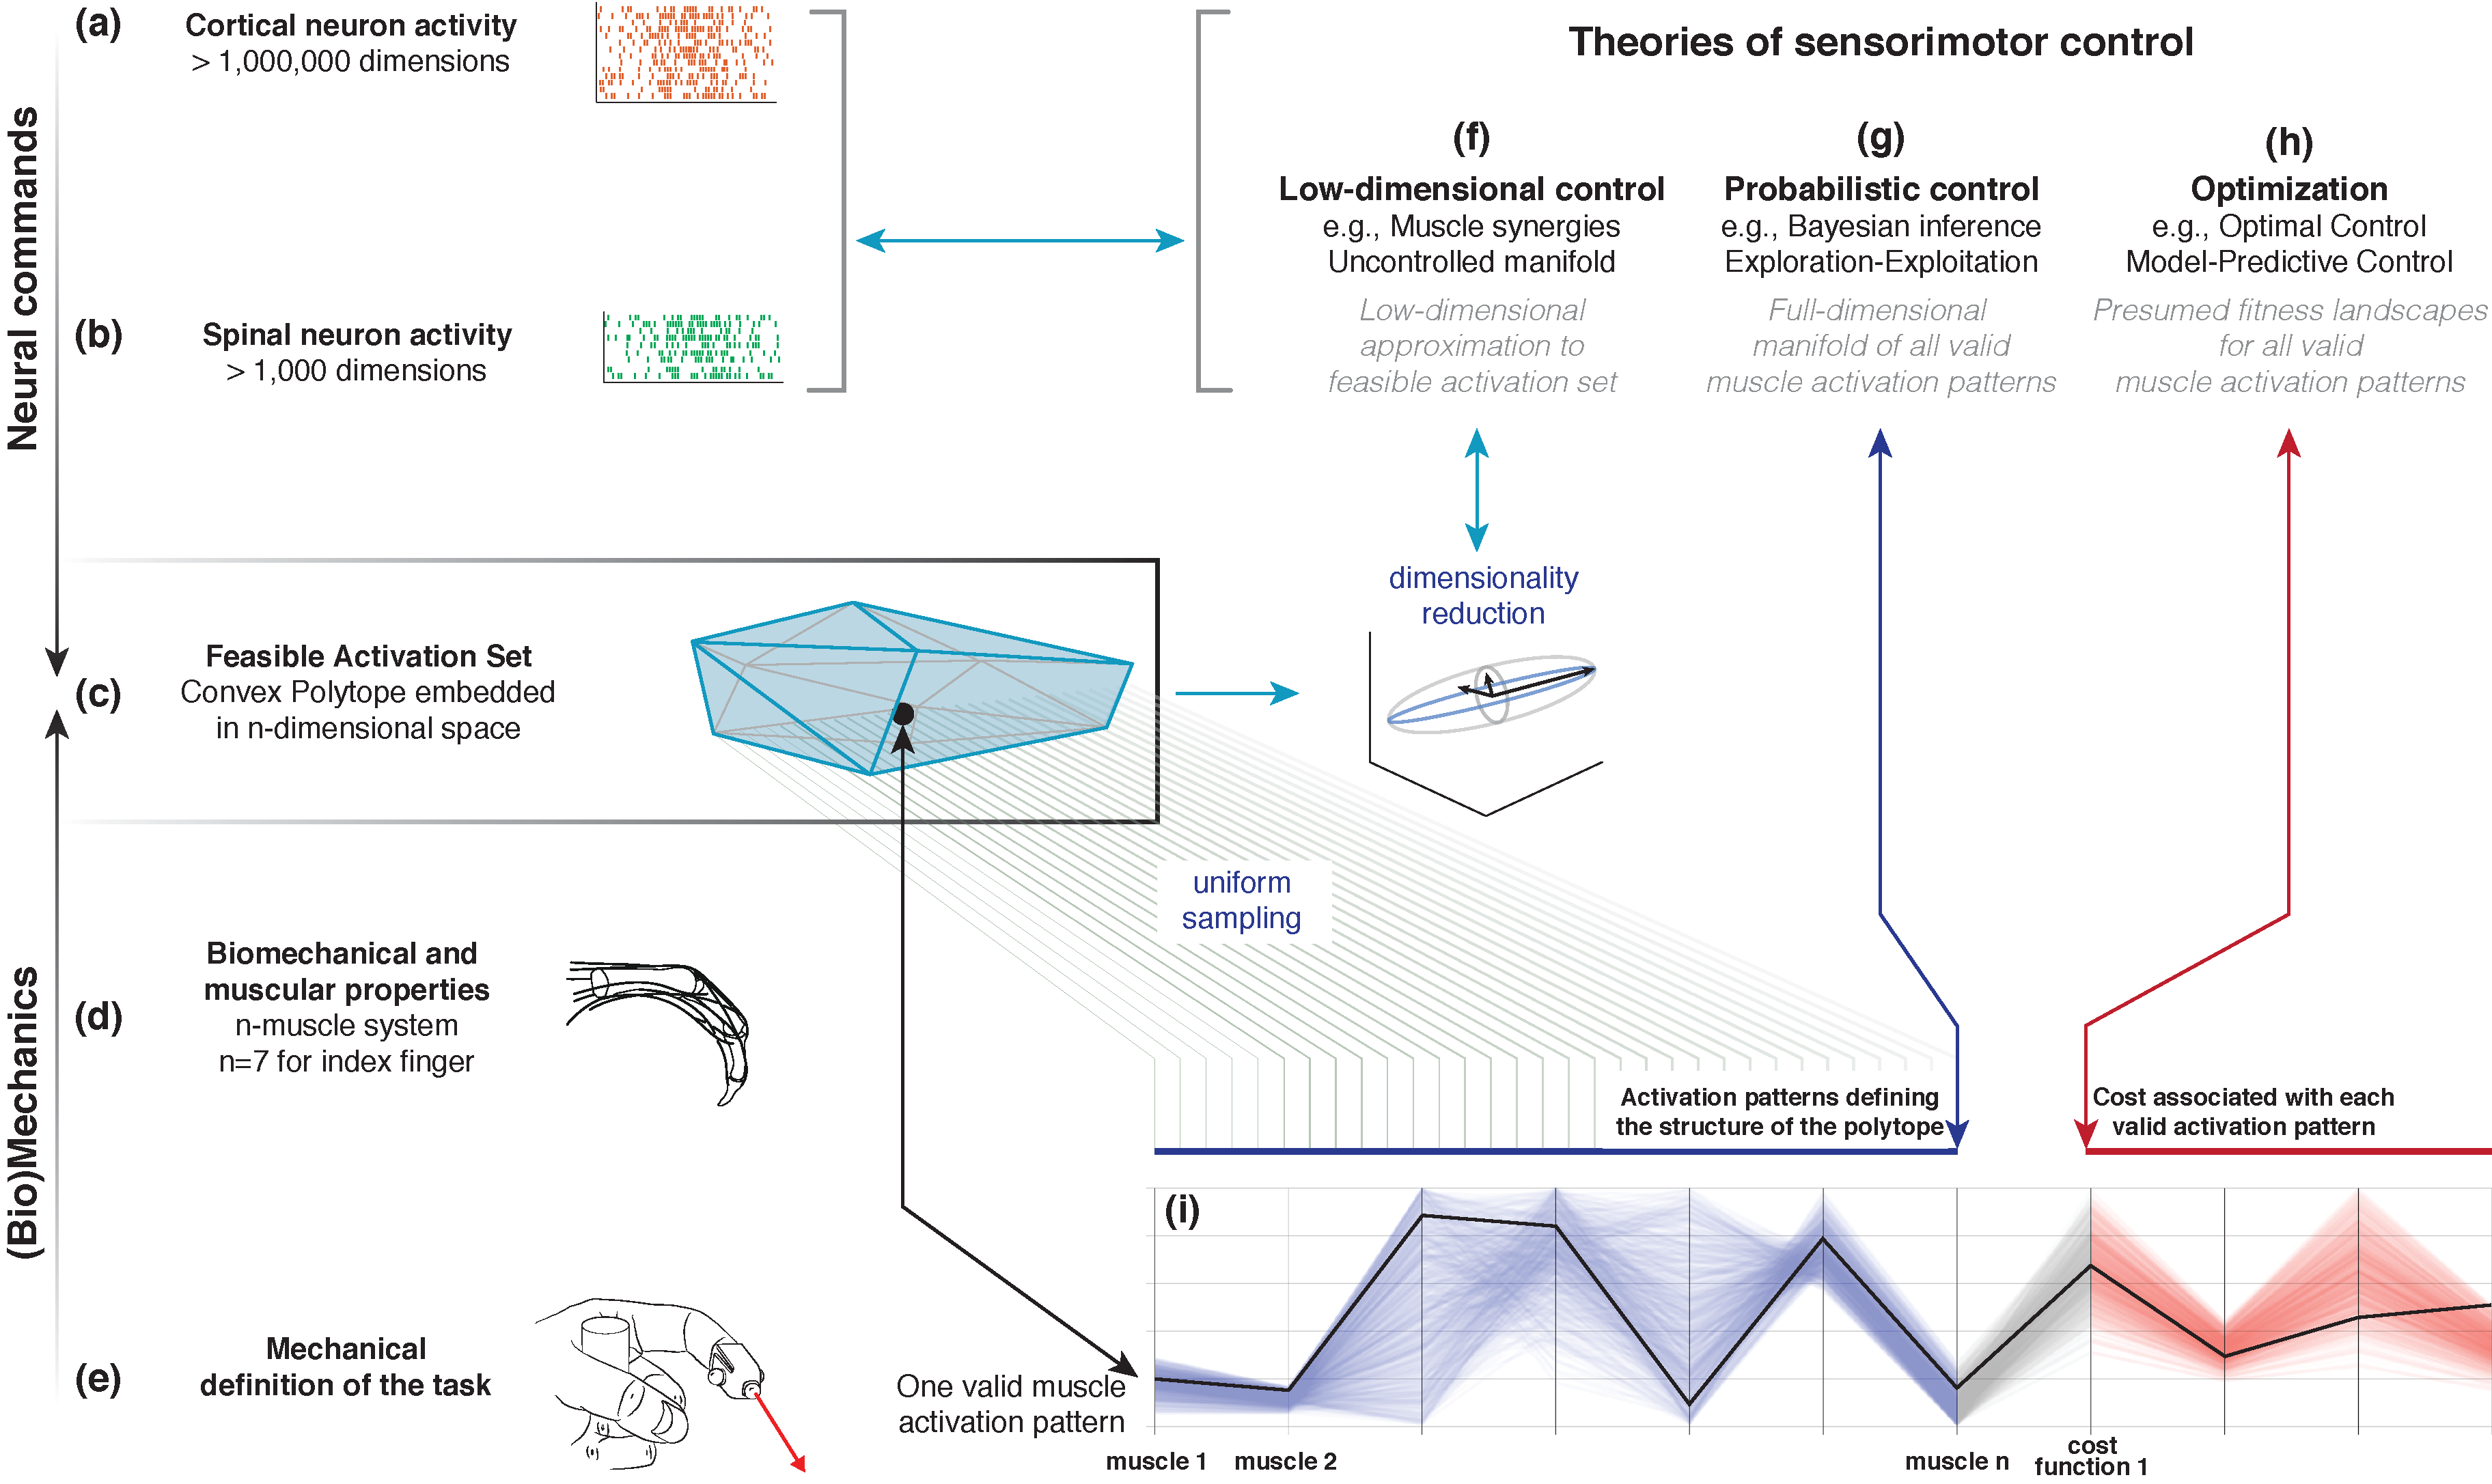
\includegraphics[width=1.0\textwidth]{numbered_figures/figure_1_overview.pdf}
\caption{Feasible activation sets for a motor task. The descending command for a motor task is issued by upper motor neurons in primary motor cortex (a), which project onto the spinal cord via the cortico-spinal tract to drive $alpha$-motor neurons (b). The combined drive to all $alpha$-motor neurons of a muscle can be considered the level of activation to that muscle.  If we consider that a motor command is sent to all relevant muscles simultaneously, then the resulting motor command is a  multi-dimensional muscle activation pattern (i.e., a point) in a high-dimensional muscle activation space \cite{Chao1978Graphical, spoor1983balancing, Kuo1993Human, Valero-Cuevas1998Large} (c). For that muscle activation pattern to be a valid solution, it must satisfy the mechanical requirements of the task (f), given biomechanical capabilities of the limb (e). Given the large number of muscles in vertebrates, there is muscle redundancy in the sense that there is an infinite number of valid solutions. We now present what to our knowledge is the first detailed description of all valid solutions (the structure of the feasible activation set, (d)), which allows to us to compare, contrast and reconcile today's three dominant approaches to motor control (g, h, i).}
\label{fig:overview}
\end{figure}

\begin{figure}[htbp]
\centering
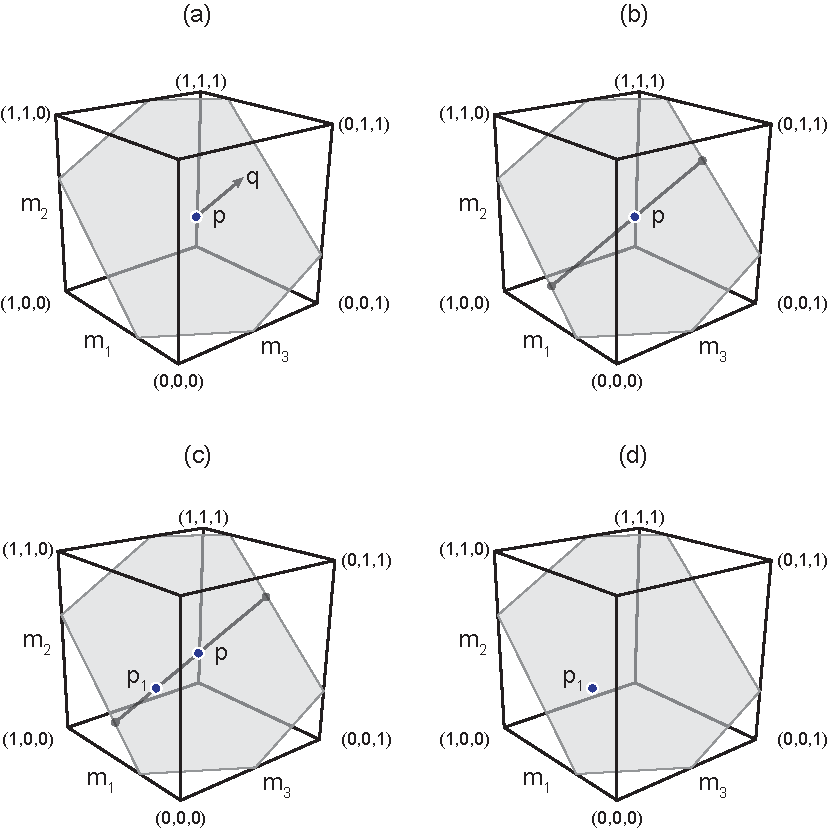
\includegraphics[width=0.5\textwidth]{numbered_figures/figure_2_hit_and_run_steps.pdf}
\caption{Graphical description of the Hit-and-Run algorithm.}
\label{fig:figure_2_hit_and_run_steps}
\end{figure}

\begin{figure}[htbp]
\centering
\includegraphics[width=0.5\textwidth]{numbered_figures/figure_3_hit_and_run_result.pdf}
\caption{Points from the solution space.}
\label{fig:figure_3_hit_and_run_result.pdf}
\end{figure}

\begin{figure}[htbp]
  \centering
  \includegraphics[width=1.0\textwidth]{numbered_figures/figure_4_parcoord_schematic.pdf}
  \caption{Parallel coordinates visualization of valid muscle activation patterns. (a) Consider three valid points (i.e., muscle activation patterns) belonging to the 2-D polytope of the feasible activation set embedded in 3-D.  (b) Activation levels (i.e., coordinates) for each point sown in parallel coordinates format. (c) The associated cost of each muscle activation pattern as per three representative cost functions.
The activation levels are bound between $0$ and $1$, and cost are normalized to the observed range of each cost.}
  \label{fig:points_to_parcoords_mapping}
\end{figure}


\begin{figure}[htbp]
\centering
\includegraphics[width=\textwidth]{numbered_figures/figure_5_parcoord.pdf}
\caption{parallel coordinates!}
\label{fig:figure_5_parcoord}
\end{figure}



\begin{figure}[htbp]
\centering
\includegraphics[width=\textwidth]{numbered_figures/figure_6_histogram_heatmap.pdf}
\caption{Density distributions converging as the output task approaches maximal distal force. Color indicates the percentage of solutions for a given task level that landed within a given 0.05-width activation bin, for each of the seven muscles (labeled on the left). The y axis indicates activation from 0 to 1 (full activation).}
\label{fig:figure_6_histogram_heatmap}
\end{figure}


\begin{figure}[htbp]
\centering
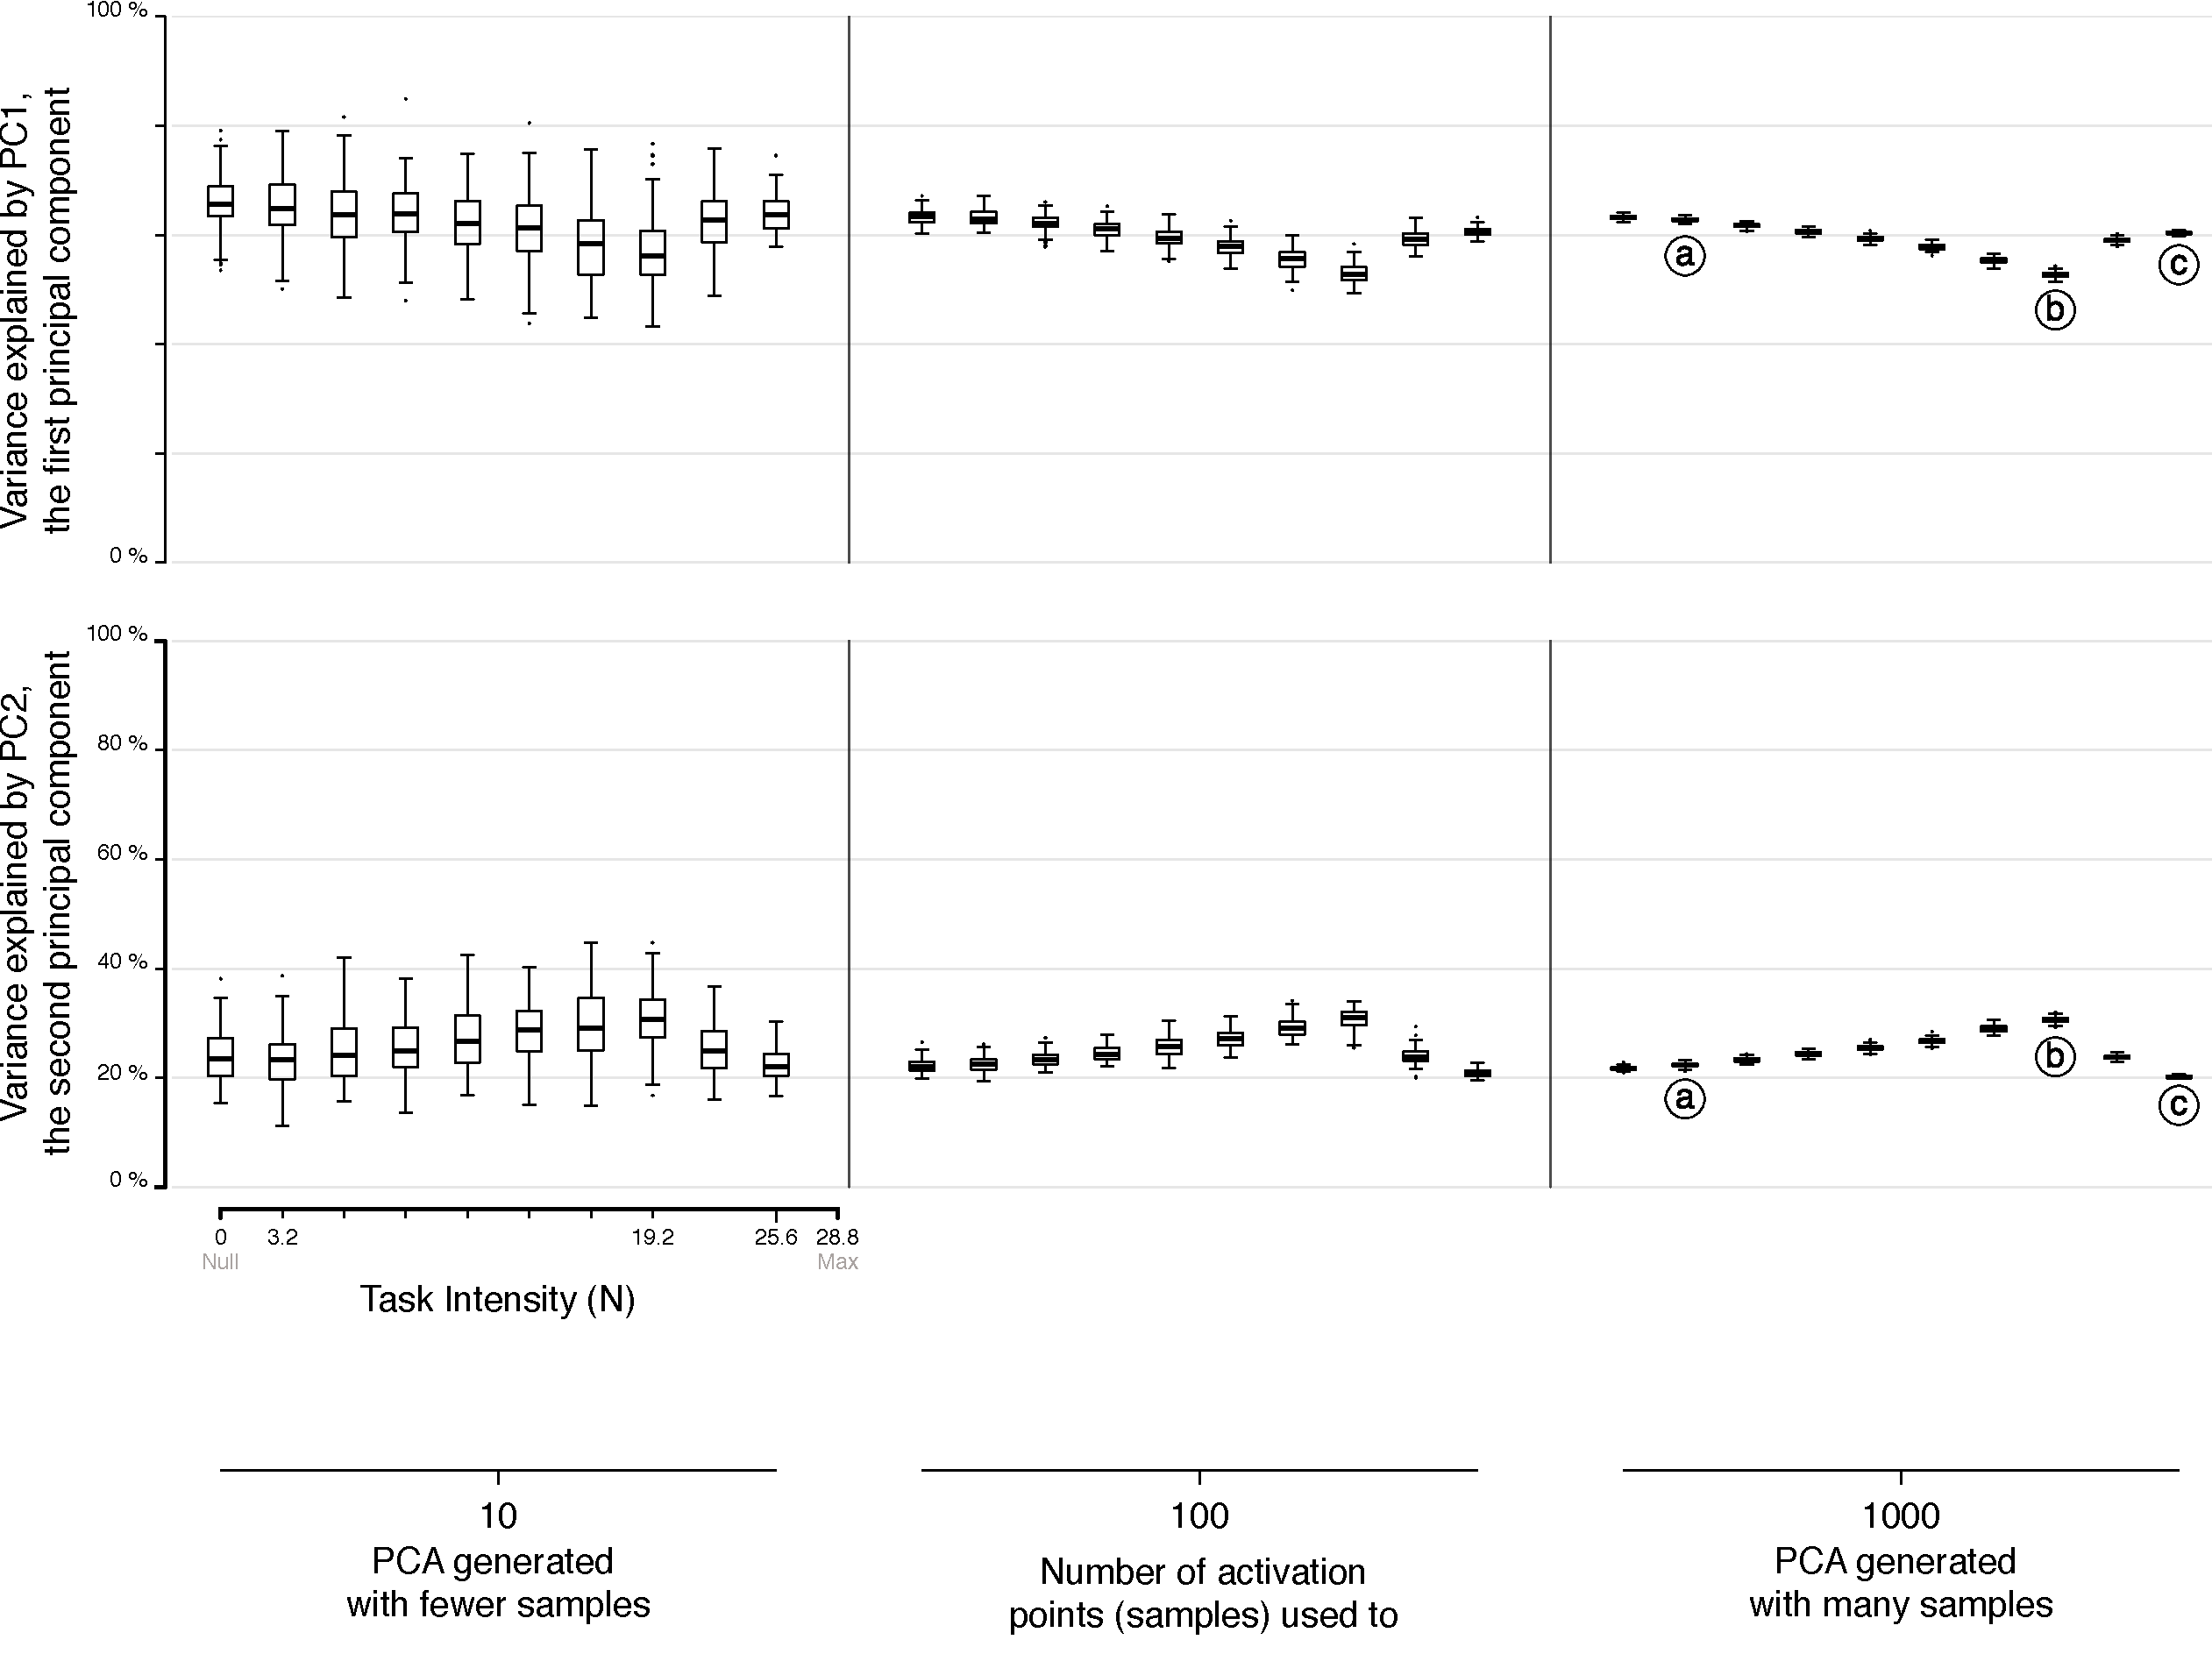
\includegraphics[width=\textwidth]{numbered_figures/figure_7_pca_variance_explained.png}
\caption{As more points are sampled from the activation space, the more clearly we can see a shift in the lower dimensional understanding of the space.}
\label{fig:pca_variance_explained}
\end{figure}
\begin{figure}[htbp]
\centering
\includegraphics[width=\textwidth]{numbered_figures/figure_8_pca_loadings.pdf}
\caption{The loadings change as we increase force in the distal direction.}
\label{fig:pca_loadings}
\end{figure}

%supplemental figures

\begin{figure}[h]
  \label{fig:schematic_arm}
  \centering
  \includegraphics{supplemental_figures/schematic_arm_1D.pdf}
  \caption{Supplemental Information Figure: One imagined visualization of the fabricated tendon driven system, with 3 generators.}
\end{figure}
\begin{figure}[t]
  \label{fig:polygon_slice_solution_space}
  \centering
  \includegraphics[width=0.25\textwidth]{supplemental_figures/feasibleactivation.png}
  \caption{Supplemental Information Figure: The feasible activation set for a  three-muscle system meeting one functional constraint is a polygon in $\mathbb{R}^3$.} %Note that muscle activations are assumed to be bounded between $0$ and $1$.}
\end{figure}

\end{document}

